\documentclass[11pt, letterpaper]{article}

% -------------------------------------------------------------------------
% Commands
\usepackage[utf8]{inputenc}
\usepackage{graphicx}
\usepackage{hyperref}
\usepackage{cite}
\usepackage{vmargin}
\usepackage{lipsum}
\usepackage{amsmath}

\setmargins{2.5cm}                 % margen izquierdo
{1.5cm}                            % margen superior
{16.5cm}                           % anchura del texto
{23.42cm}                          % altura del texto
{10pt}                             % altura de los encabezados
{1cm}                              % espacio entre el texto y los encabezados
{0pt}                              % altura del pie de página
{2cm}                              % espacio entre el texto y el pie de página

% \hyphenation{}

% \hypersetup{colorlinks,%
% 	citecolor=blue,%s
% 	filecolor=blue,%
% 	linkcolor=blue,%
% 	urlcolor=blue%
% }


% -------------------------------------------------------------------------
\title{\textbf{Simulating Cross-Feeding Dynamics Using Proteome-Constrained FBA}}

% -------------------------------------------------------------------------

\date{}
\author{
  % \textbf{Jos\'e A. Pereiro-Morej\'on$^{1,3}$, Roberto Mulet$^{1,2}$} \\
  % \small{1. Group of Complex Systems and Statistical Physics.} \\
  % \small{Physics Faculty, University of Havana, CP 10400. La Habana, Cuba} \\
  % \small{2. Department of Theoretical Physics, }\\
  % \small{Physics Faculty Faculty, University of Havana, CP 10400. La Habana, Cuba} \\
  % \small{3. Biology Faculty, University of Havana, CP 10400. La Habana, Cuba} \\
}

% -------------------------------------------------------------------------
% opening
\begin{document}

\maketitle

% \begin{abstract}
% 	\lipsum[2]
% \end{abstract}


% MARK: Protein Allocation Models
\section{Protein Allocation Models}

Protein Allocation Models extend classical constraint-based models of genome-scale metabolic networks by introducing constraints that reflect condition-dependent patterns of proteome allocation \cite{moriConstrainedAllocationFlux2016, alterProteomeRegulationPatterns2021}.
Conveniently, many of the so-called "growth laws" \cite{scottBacterialGrowthLaws2011} can be straightforwardly integrated into the optimization frameworks where these models are typically used. 

The classical formulation of a constraint-based model is:

% MARK: ..classical problem
\begin{align*}
  \max_{v} \quad & f(v) \\
  \text{s.t.} \quad & \\ 
  & Sv = 0 \\
  & 0 \leq v \leq U
\end{align*}

where $v$ is the flux vector across the network, $U$ are their upper bounds, $S$ is the stoichiometric matrix and $f$ the objective function (eg: biomass production). 

To incorporate growth condition-dependent proteome allocation, we must link proteome fractions to the flux variables.
This is feasible because most reactions in the network are mediated by proteins (enzymes and transporters).
For instance, Alter et al.~\cite{alterProteomeRegulationPatterns2021} proposed the following model:

% MARK: ..PAM problem
\begin{align*} 
\max_{v} \quad & f(v) \\
\text{s.t.} \quad & \\ 
& Sv = 0 \\
& 0 \leq v \leq U \\
& \phi_{T} = \phi_{T, 0} + \omega_{T} * \mu \\
& \phi_{UE} = \phi_{UE, 0} - \omega_{UE} * u \\
& \phi_{AE} = \sum_{e} \frac{M_e}{k_{cat, e}}  * v_e \\
& \phi_{T} + \phi_{UE} + \phi_{AE} \le 0.26 \text{ g/gCDW}
\end{align*}

These relationships between proteome fractions ($\phi_*$) and flux variables are derived from experimental and biochemical data.
For instance, Figure \ref{fig:proteome-allocation-patterns} illustrates the growth-dependent relationships for $\phi_{T}$ (transational related proteome fraction) and $\phi_{UE}$ ('unused' enzymes proteome fraction). 

In short, $\phi_{T}$ is assumed to vary linearly with the growth rate ($\mu \in v$), $\phi_{UE}$ with the uptake of the limiting nutrient ($u \in v$), and $\phi_{AE}$  (active enzymes proteome fraction) with the linear combination of enzymatic fluxes ($v_e \in v$) where $M_e$ and $k_{cat, e}$ are the effective molecular weight and catalytic constant of enzyme $e$, respectively.
The total proteome fraction is bounded by an experimentally determined value.
See further details at \cite{alterProteomeRegulationPatterns2021}.

It is convenient that these constraints can be expressed as linear relations, allowing the use of efficient linear programming algorithms.

\begin{figure}
	\centering
	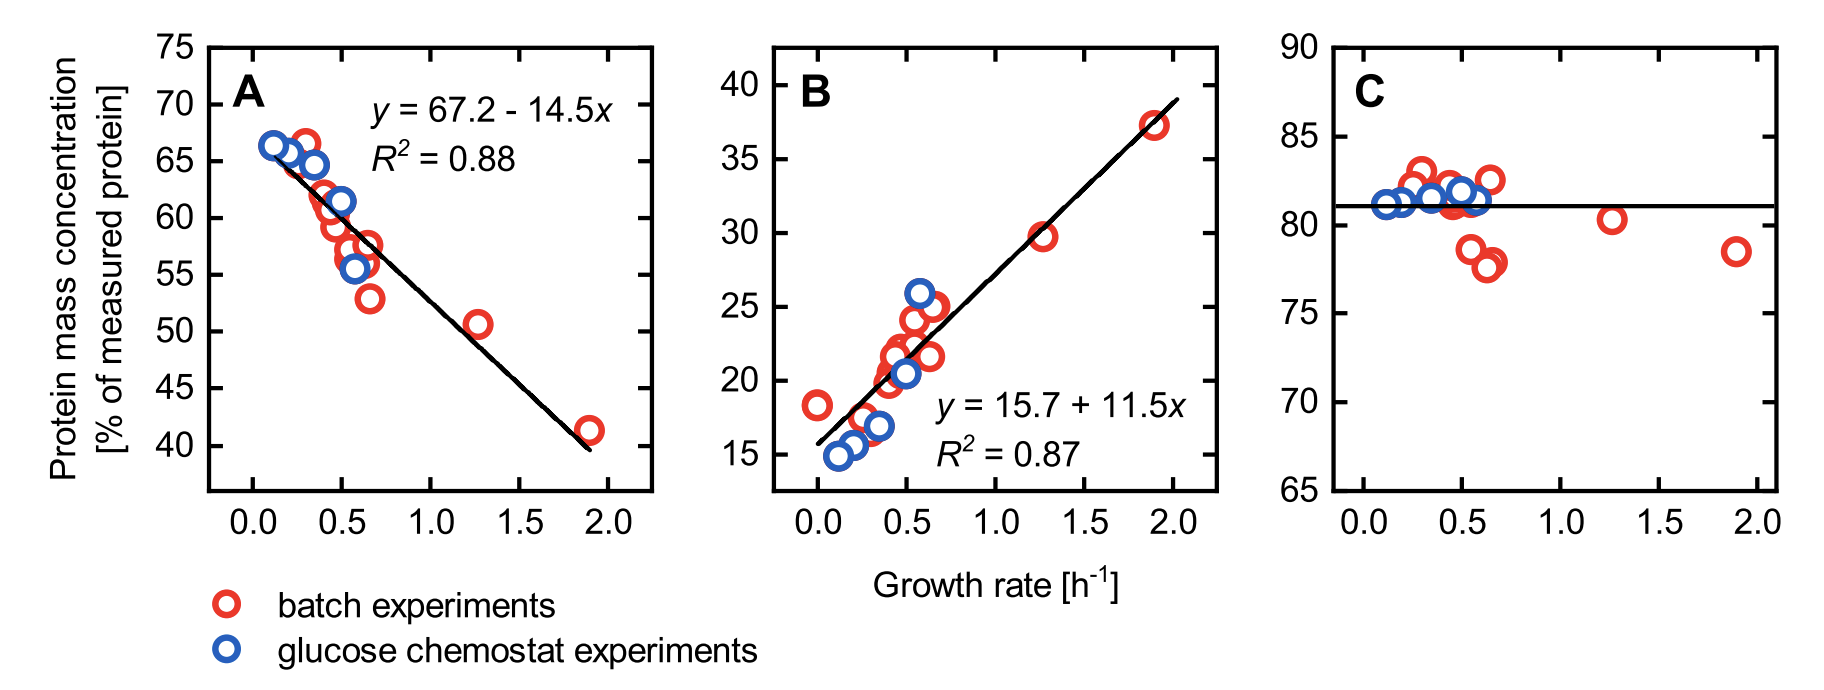
\includegraphics[scale = 0.5]{images/proteome-allocation.png}
	\caption{
		\textbf{Protein mass data of distinct protein sectors under diverse growth conditions taken from Schmidt et al. \cite{schmidtQuantitativeConditiondependentEscherichia2016}}:
    (A) All proteins represented by the iML1515 GEM and found in the proteomic data set, comprising the active and unused enzymes sectors. (B) Translational sector covering proteins assigned to the COG (Clusters of Orthologous Groups) class "translation, ribosomal structure, and biogenesis," which are not included in the iML1515. The black lines in panels A and B are linear fits of the data points resulting in the shown equations and coefficients of determination R2 . (C) Sum of the protein mass concentrations shown in panels A and B. The horizontal black line marks the 81\% of measured protein mass used to constrain protein availability in the PAM. Glucose chemostat and batch experiments are highlighted in blue and red, respectively. Note that protein concentrations relative to the cell dry weight (cdw) were related to the total protein concentration of 0.32 $g\,g^{-1}_{cdw}$ measured by Schmidt et al \cite{schmidtQuantitativeConditiondependentEscherichia2016}.
    \textbf{Both figure and caption taken from \cite{alterProteomeRegulationPatterns2021}}.
	}
	\label{fig:proteome-allocation-patterns}
\end{figure}


% MARK: Coexistence model
\section{Coexistence model}

We can extend the proteome allocation model described above to include two distinct stoichiometric matrices, one for each auxotrophic strain.
Figure \ref{fig:PAM-S-schema} descirbe the model general layout. 
A key feature is that the two networks interact only through the medium; no direct interaction between strains is modeled.
This allows independent control of the exchange reactions for each strain.
This can be achieved by adding extra reactions and metabolites that model the mass flux to/from the 'medium', and to/from the 'universe'.

\begin{figure}
	\centering
	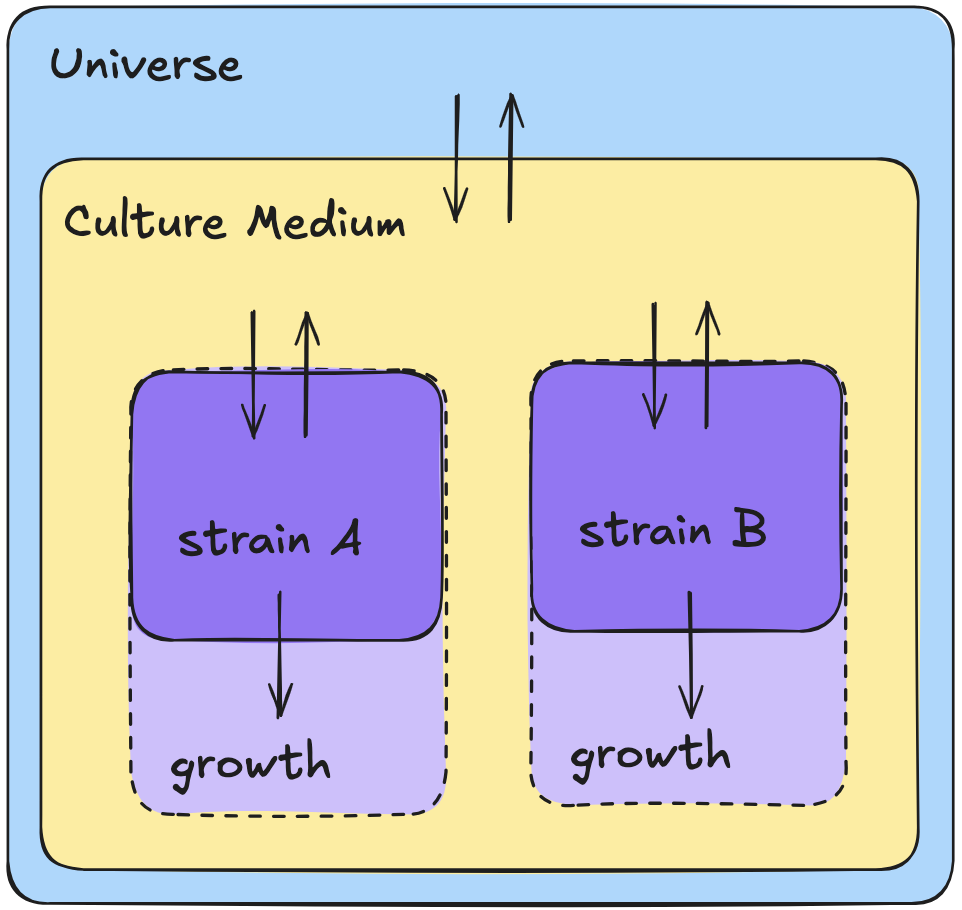
\includegraphics[scale = 0.5]{images/PAM-S-schema.png}
	\caption{
		\textbf{Schema of a mixed model}: Arrows indicate mass fluxes. Note that strains can only interact by its influence with the medium. 
	}
	\label{fig:PAM-S-schema}
\end{figure}

% MARK: DFBA
\section{DFBA: Coexistence in a Chemostat}

Proteome allocation models show significantly improved ability to predict the physiological behavior of E. coli cultures compared to standard stoichiometric models \cite{alterProteomeRegulationPatterns2021}. 
This motivates evaluating their performance in the context of coexistence.
To that end, we use dynamic flux balance analysis (DFBA) to simulate a chemostat culture of E. coli auxotrophs engineered to engage in forced cross-feeding of essential amino acids.

For simplicity, the simulations only track the dynamics of the cell densities ($X_*$) and the single carbon source ($s_{glc}$). 
The carbon source uptake is modeled using the standard Michaelis-Menten kinetics:

\begin{align*} 
  U_{\text{intake glc}} = V^{max}_{glc} * \frac{s_{glc}}{KM_{glc} + s_{glc}}
\end{align*} 

note that $U_{glc}$ will be common for all strains. 

Any component of the medium supplied by the 'universe' is considered infinitely available, and its dynamics are therefore neglected.
Additionally, nutrients produced by the strains are assumed to be non-accumulating.
That is, at any moment, each strain can consume only what the other is producing, in proportion to their respective cell densities.
For a metabolite $k$ we have:

\begin{align*} 
  v_{\text{intake k}}^{\text{strain A}} \le
  v_{\text{production k}}^{\text{strain B}} * 
  \frac{X^{\text{strain B}}}{X^{\text{strain A}}} 
\end{align*} 

With this setup, we can simulate the dynamics of a chemostat culture:

\begin{align*} 
  \frac{X^*(t+1) - X^*(t)}{\Delta t} &= 
  (\mu - D) * X^*(t) 
  \\
  \frac{s_{glc}(t+1) - s_{glc}(t)}{\Delta t} &= 
  (c_{glc} - s_{glc}(t)) * D + 
  \sum_i (v^i_{\text{production k}} - v^i_{\text{intake k}}) * X^{\text{strain i}}
\end{align*} 

where the sum is over all strains and $X^*$ is the cell density of a given strain.
The fluxes $\mu$ and $v^*_*$ are computed by solving an FBA problem contextualized by the current concentration and production of nutrients. 

\section{Results}


We simulate co-cultures of two E. coli auxotrophs: $\Delta$Ile, which cannot produce isoleucine, and $\Delta$Met, which cannot produce methionine.

Because the appropriate objective function is unclear, we evaluate several alternatives. Each objective function is a linear combination of fluxes and can be parameterized by the choice of coefficients.

We used the follow linear objective function:

\begin{itemize}

  \item \textbf{$\Delta$Ile.egoist.max.yield}:
  We use coefficients spanning different orders of magnitude to setup a hierarchical optimization. In this case the objective function will be:
  \begin{align*} 
    f(v) = & 
    10^{4} \mu^{\Delta Ile} + 10^{2} \mu^{\Delta Met} \\
    & - 10^{-4} v^{\Delta Ile}_{\text{intake gluc}} - 10^{-4} v^{\Delta Met}_{\text{intake gluc}} \\
    & - 10^{-4} v^{\Delta Ile}_{\text{intake Ile}} - 10^{-4} v^{\Delta Met}_{\text{intake Met}}
  \end{align*} 
  This formulation tends to maximize both biomass production rates while minimizing nutrient intake. 
  However, due to the large differences in coefficient magnitudes, the optimizer will prioritize the higher-weighted terms.
  
  \item \textbf{$\Delta$Met.egoist.max.yield}
  Analogous to the previous one but changing the biomass coeffitients so mutant $\Delta$Met is prioritized. 
  The rest is identical to the first objective function.
  \begin{align*} 
    f(v) = & 
    10^{2} \mu^{\Delta Ile} + 10^{4} \mu^{\Delta Met} \dots
  \end{align*} 

  \item \textbf{$\Delta$Ile.egoist.only}:
  This time the only biomass flux being optimized (maximized) is the biomass rate of the $\Delta$Ile mutant. 
  The rest is identical to the first objective function.
  \begin{align*} 
    f(v) = & 
    10^{4} \mu^{\Delta Ile} + 0.0 \mu^{\Delta Met} \dots
  \end{align*} 
  
  \item \textbf{$\Delta$Met.egoist.only}:
  Analogous to the previous one but for the $\Delta$Met mutant.
  The rest is identical to the first objective function.
  \begin{align*} 
    f(v) = & 
    0.0 \mu^{\Delta Ile} + 10^{4} \mu^{\Delta Met} \dots
  \end{align*} 

  \item \textbf{non-competitive.max.yield}
  In this case, both biomasses have equal weight in the optimization.
  The rest is identical to the first objective function.
  \begin{align*} 
    f(v) = & 
    10^{4} \mu^{\Delta Ile} + 10^{4} \mu^{\Delta Met} \dots
  \end{align*} 

\end{itemize}

\begin{figure}
	\centering
	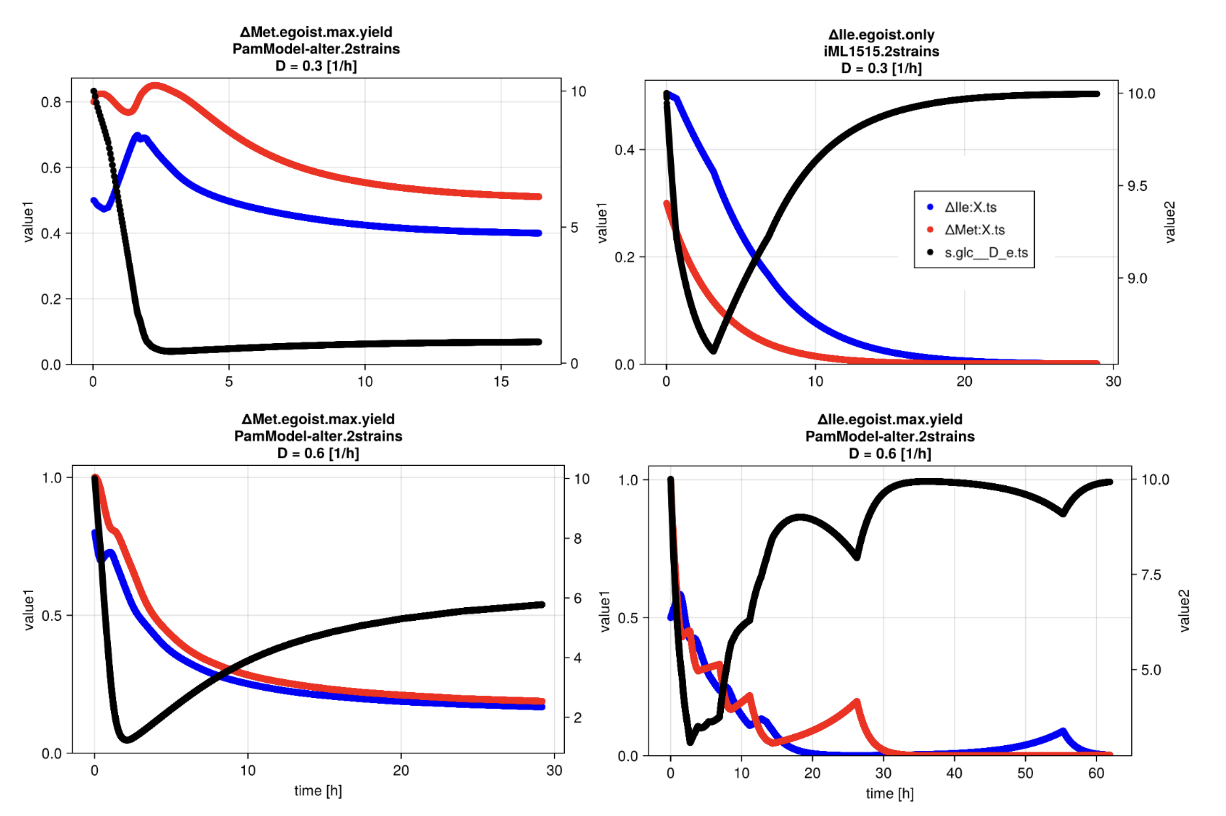
\includegraphics[scale = 0.7]{images/dym-ts.png}
	\caption{
		\textbf{Representative dynamic simulations}: The plots show the evolution of cell density (right y-axis) and glucose concentration in the medium (left y-axis) under different conditions.
	}
	\label{fig:dym-ts}
\end{figure}

Figure \ref{fig:dym-ts} shows representative dynamics for cell densities and residual glucose concentration. In most cases, the dynamics are smooth, but at high dilution rates they may become unstable (see bottom left panel). These unstable simulations are excluded from analysis.

Another observation is that all simulations with \textbf{$\Delta$*.egoist.only} objective functions failed to achieve coexistence.
This is likely because maximizing the growth of only one strain (the egoist) results in no flux being allocated to the other strain's biomass, leading to its eventual washout.
This, in turn, limits the egoist's access to the essential metabolite it depends on, preventing it from maintaining growth above the dilution rate. 
The top-right panel of Figure \ref{fig:dym-ts} illustrates this scenario.

\begin{figure}
	\centering
	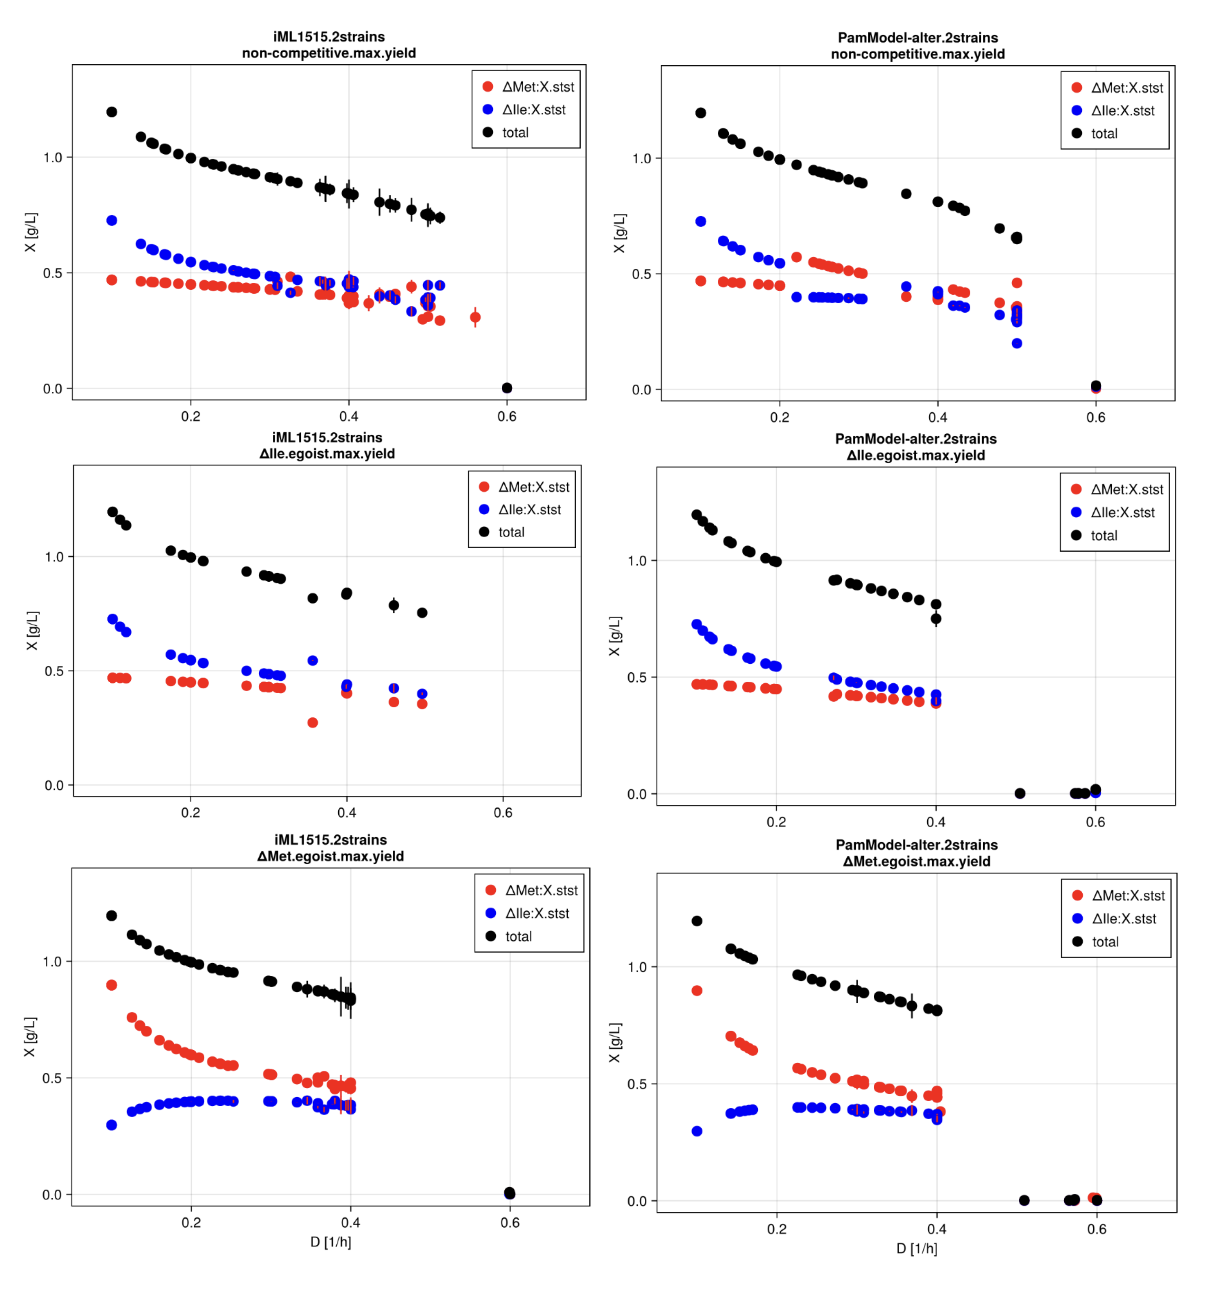
\includegraphics[scale = 0.7]{images/stst-X-Ds.png}
	\caption{
		\textbf{Steady-state cell densities}: 
    Results are shown for both the proteome allocation model (PamModel-alter.2strains) and the baseline model (iML1515.2strains) without proteome allocation constraints. Only simulations where cell densities remained stable ($\pm$ 20\%) during the final 10\% of the time window are included. Error bars indicate this variation.
	}
	\label{fig:stst-X-Ds}
\end{figure}

\begin{figure}
	\centering
	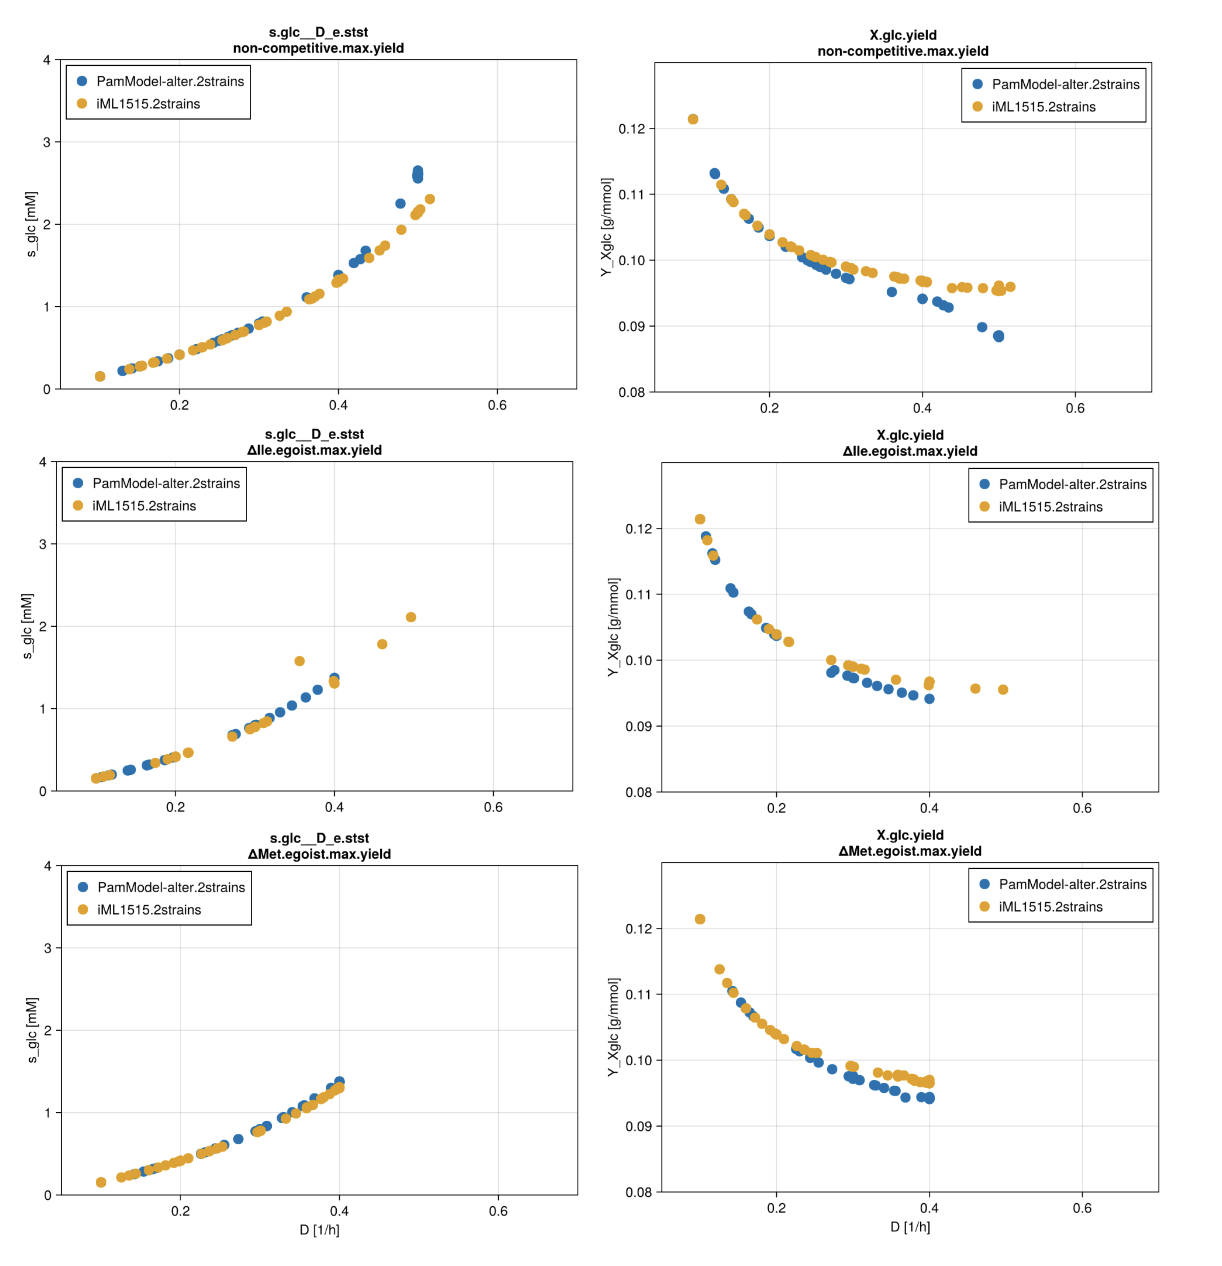
\includegraphics[scale = 0.7]{images/stst-sglc-YXglc-Ds.png}
	\caption{
		\textbf{Steady-state glucose levels and biomass yield}: 
    This figure parallels Figure \ref{fig:stst-X-Ds} but reports residual glucose concentration (mM) and biomass yield (g/mmol glucose).
	}
	\label{fig:stst-sglc-YXglc-Ds}
\end{figure}

Figures \ref{fig:stst-X-Ds} and \ref{fig:stst-sglc-YXglc-Ds} show the results for the simulations that reached a stady state. 
From the figures, we can make the following observations:

\begin{itemize}
    \item 
    The total culture biomass decreases as the dilution rate (D) increases ((Figure \ref{fig:stst-X-Ds})). 
    \item 
    At higher dilution rates, the steady-state cell densities of both mutants tend to converge ((Figure \ref{fig:stst-X-Ds})). 
    \item 
    The selection of objective function affects the initial difference of steady state cell density at low dilution rate. 
    \item 
    Biomass yield (g biomass per mmol glucose) declines with increasing D (Figure \ref{fig:stst-sglc-YXglc-Ds})
    
\end{itemize}


% ΔIle:BIOMASS_Ec_iML1515_WT_75p37M_f
% (-0.149336) met__L_c
% (-0.282306) ile__L_c


% MARK: ..Next
\section{Further Considerations}

\begin{itemize}
  \item 
  Identify interesting questions that can be addressed using genome-scale metabolic models, which cannot be captured by simpler dynamic models.
  
  \item 
  Consider incorporating the effect of antibiotics, as described by another "growth law" \cite{grilli2025notes}, and investigate its impact on coexistence.
  For example, what happens if only one strain is sensitive while the other is resistant?
  
  \item 
  From an experimental perspective, all these experiments are feasible using the DIY chemostat setup.
\end{itemize}


\bibliographystyle{plain}
\bibliography{main}
	
\end{document}
